\chapter{Current Research Achievements} % Main chapter title

\label{Current Research Achievements} % For referencing the chapter elsewhere, use \ref{Chapter1} 

\section{ScTI Methods are Constantly Being Developed}

In the past few years, single-cell omics technology has flourished, and more and more scTI methods have been invented. Every month, new scTI methods are published, and researchers from around the world are continually experimenting with these new methods to get the most complete cell map. In the repository of commonly used single-cell omics tools \parencite{henry_omictools:_2014,davis_seandavi/awesome-single-cell:_2018,zappia_exploring_2018}, it is not difficult to find that the scTI tool is one of the largest categories of current single-cell omics tools. The core algorithms of each scTI are different, which means that the prior knowledge they rely on and their inferable trajectory structures are dissimilar. Also, different methods often have their own unique output structure.

\section{ScTI Methods Analyzing Different Cell Lineage}

Current computational methods have proven useful for analyzing cell lineage and corresponding trajectories based on large numbers of single-cell omics data, but these strategies still have limitations on many issues. We need better algorithms to derive multi-branched structures, to achieve more efficient extraction of cell features, and to take into account multiple pathways in order to show the fact that the same cell in a cell lineage may follow multiple dynamic paths simultaneously \parencite{ferrell_bistability_2012}. In the study of cell lineage with simple topologies, researchers have achieved many results, such as inferring cell lineage during differentiation of B cells by single-cell proteomic data 
\parencite{bendall_single-cell_2014}, and studying the lineage of nervous system development
\parencite{habib_div-seq:_2016,chen_mpath_2016,shin_single-cell_2015} and early hematopoietic process
\parencite{nestorowa_single-cell_2016} with single-cell transcriptome data. \\

Of course, in more complex cell differentiation systems, cell lineage constructed using single-cell omics can also reveal the answers to important biological questions. Studies of embryonic stem cells have helped us understand embryonic development at the cellular level and find marker molecules for different cells at specific stages of embryonic development
\parencite{haghverdi_diffusion_2016,haghverdi_diffusion_2015}. Researchers who focus on bone marrow cells solve the problem that has plagued the academic world for many years through the method of single-cell omics: whether hematopoietic stem cells in the bone marrow have differentiated preferences after maturity and tend to differentiate to a certain kind of cell ? \parencite{paul_transcriptional_2015,olsson_single-cell_2016} 

\subsection{Hematopoietic System}

Previous studies have shown that in the hematopoietic system, the use of scTI methods to infer cell lineage is quite appropriate. In the single-cell data on hematopoietic cells, the researchers accurately isolated hematopoietic stem cells and progenitor cells (HSPCs) from single-cell data from acute myeloid leukemia by analyzing data from normal hematopoietic cells. This method is more accurate than traditional methods. Because traditional methods are based on classical cell surface markers, in some cases, such strategies do not accurately identify diseased cells in a disease. Single-cell omics data provides ultra-high-dimensional feature information, which makes feature-based recognition more accurate \parencite{levine_data-driven_2015}.

\subsection{Cancer Research}

Single-cell omics has revolutionized the entire field of cancer research. In the field of single cells just introduced into cancer research, qPCR-based single cell methods have been used to study radiation resistance of cancer cells and heterogeneity of colon cancer tissues at the cellular level 
\parencite{diehn_association_2009, dalerba_single-cell_2011}. With the rise of second-generation sequencing technology, single-cell omics analysis provides new tools for researchers studying breast cancer and acute lymphoblastic leukemia \parencite{wang_clonal_2014, gawad_dissecting_2014}. On this basis, researchers can also infer the order in which various mutations lead to cell carcinogenesis \parencite{corces-zimmerman_preleukemic_2014,jan_clonal_2012}. \\

Analysis of single-cell RNA-seq data from some fresh tumor tissues can distinguish epithelial cells, immune cells, stromal cells and cancer cells. This method has achieved very good results in melanoma \parencite{tirosh_dissecting_2016}, myeloproliferative neoplasms \parencite{kiselev_sc3:_2017} and glioblastoma \parencite{patel_single-cell_2014}. Among the identified cancer cells, single-cell transcriptome data can also be used to distinguish cancer cells of different states, such as cancer stem cells 
\parencite{patel_single-cell_2014,tirosh_single-cell_2016} and resistant cancer cells 
\parencite{tirosh_dissecting_2016}. In cancer stem cells, cells in an active value-added state and cells in a relatively static state can also be identified 
\parencite{patel_single-cell_2014,tirosh_dissecting_2016,tirosh_single-cell_2016}. 

\section{Summery of Commonly Used scTI Methods}

In the next sections, I have selected 20 commonly used scTI methods and divided them into different groups according to the different characteristics of their core algorithms. These are all based on $Python$ or $R$. In Table \ref{tab:Methods} below, I listed the priori requirements, basing platform, topology features and references of these methods. In Table \ref{tab:Trajectory}, seven basic inferable trajectory types of scTI methods are defined, however, not all scTI methods are applicable to all of these topologies. When it comes to Figure \ref{fig:Trajectory}, these inferable trajectory types of scTI methods are represented in cartoons. Last, I show the inferable trajectory types of every scTI method in Table \ref{tab:Inferable Trajectory}. \\

These methods are different from each other and have their own characteristics. In the course of practical research, researchers tend to combine results from multiple methods in order to achieve a satisfying end result.

\subsection{Commonly Used scTI Methods}

\begin{spacing}{1.15}
\begin{table}[H]
\caption{Commonly Used scTI Methods}
\label{tab:Methods}
\centering
\begin{tabular}{p{4cm} p{3cm}<{\centering} *{3}{p{2cm}<{\centering}}}
\toprule
\tabhead{Method} & \tabhead{Topology} & \tabhead{Priori} & \tabhead{Platform} 
& \tabhead{Reference} \\
\midrule
\multicolumn{2}{l}{\keyword{Tree}} \\
Monocle\_1   & Flexible   & $\vartriangle$   & $R$      &\parencite{trapnell_dynamics_2014}\\
Monocle\_2   & Unfettered &                  & $R$      &\parencite{qiu_reversed_2017}\\
Slingshot    & Unfettered &                  & $R$      &\parencite{street_slingshot:_2018}\\
MST          & Unfettered &                  & $R$      &$R^*$\\
SCUBA        & Unfettered &                  & $Python$ &\parencite{marco_bifurcation_2014}\\
pCreode      & Unfettered &                  & $Python$ &\parencite{herring_unsupervised_2018}\\
\midrule
\multicolumn{2}{l}{\keyword{Linear}} \\
Embeddr      & Constant   &                  & $R$      &\parencite{campbell_laplacian_2015}\\
TSCAN        & Constant   &                  & $R$      &\parencite{ji_tscan:_2016}\\
SCORPIUS     & Constant   &                  & $R$      &\parencite{cannoodt_scorpius_2016}\\Component\_1 & Constant   &                  & $R$      &$R^*$\\
MATCHER      & Constant   &                  & $Python$ &\parencite{welch_matcher:_2017}\\
\midrule
\multicolumn{2}{l}{\keyword{Multi-diverging}} \\
STEMNET      & Flexible   & $\blacktriangle$ & $R$    &\parencite{velten_human_2017}\\
MFA          & Flexible   & $\vartriangle$   & $R$    &\parencite{campbell_probabilistic_2017}\\
FateID       & Flexible   & $\blacktriangle$ & $R$    &\parencite{herman_fateid_2018}\\
\midrule
\multicolumn{2}{l}{\keyword{Bi-diverging}} \\
DPT          & Constant   &                  & $R$      & \parencite{haghverdi_diffusion_2016}\\
Wishbone     & Flexible   & $\vartriangle$   & $Python$ & \parencite{bendall_single-cell_2014}\\
\midrule
\multicolumn{2}{l}{\keyword{Graph}} \\
RaceID       & Unfettered &                  & $R$      & \parencite{grun_novo_2016} \\
PAGA         & Unfettered & $\vartriangle$   & $Python$ & \parencite{wolf_paga:_2019} \\
\midrule
\multicolumn{2}{l}{\keyword{Cyclic}} \\
EIPiGraph    & Constant   &                  & $R$      & $**$ \\
Angle        & Constant   &                  & $R$      & $R^*$ \\
% ${\rm R^{2}_{i}}$ 改成正常体
\bottomrule
\end{tabular}
\end{table}
$\vartriangle$ : Needing priori information like start or end cells in lineage.\\
$\blacktriangle$ : Needing priori information like cell clustering or time series.\\
Unfettered : Topological structures deduced form data are free.\\
Constant : Topological structures deduced form data are constant.\\
Flexible : Topological structures deduced form data depend on the parameters.\\
$R^*$ : This method could be implemented with a bit of R code. \\
$**$ : Only in \url{github.com/Albluca/ElPiGraph.R}.
\end{spacing}


\subsection{Basic Trajectory Structure Types}
\begin{spacing}{1.5}
\begin{table}[H]
\caption{The definition of basic trajectory structure types \parencite{saelens_comparison_2019}}
\label{tab:Trajectory}
\centering
\begin{tabular}{p{4cm} p{10cm}}
% \times \checkmark
\toprule
\tabhead{Types} & \tabhead{Definition} \\
\midrule
Linear &  
A graph that every node in this graph has an in-degree and an out-degree not higher than 1 and 2 nodes in this graph have degrees equal to 1.\\
\midrule
Ring & 
A graph that every node in this graph has an in-degree and an out-degree equal to 1.\\
\midrule
Tree & 
A graph that every node in this graph has an in-degree lower than 1.\\
\midrule
Mutil-diverging &  
A tree graph that every node except one in this tree graph has a degree not higher than 1.\\
\midrule
Bi-diverging &  
A mutil-diverging graph where a node with its degree equal to 3.\\
\midrule
Unconnected &
A graph where not all nodes are connected.\\
\midrule
Connected &
A graph where all nodes are connected.\\
% ${\rm R^{2}_{i}}$ 改成正常体
\bottomrule
\end{tabular}
\end{table}
\end{spacing}

\vspace{1.0cm}

\begin{figure}[H]
\centering
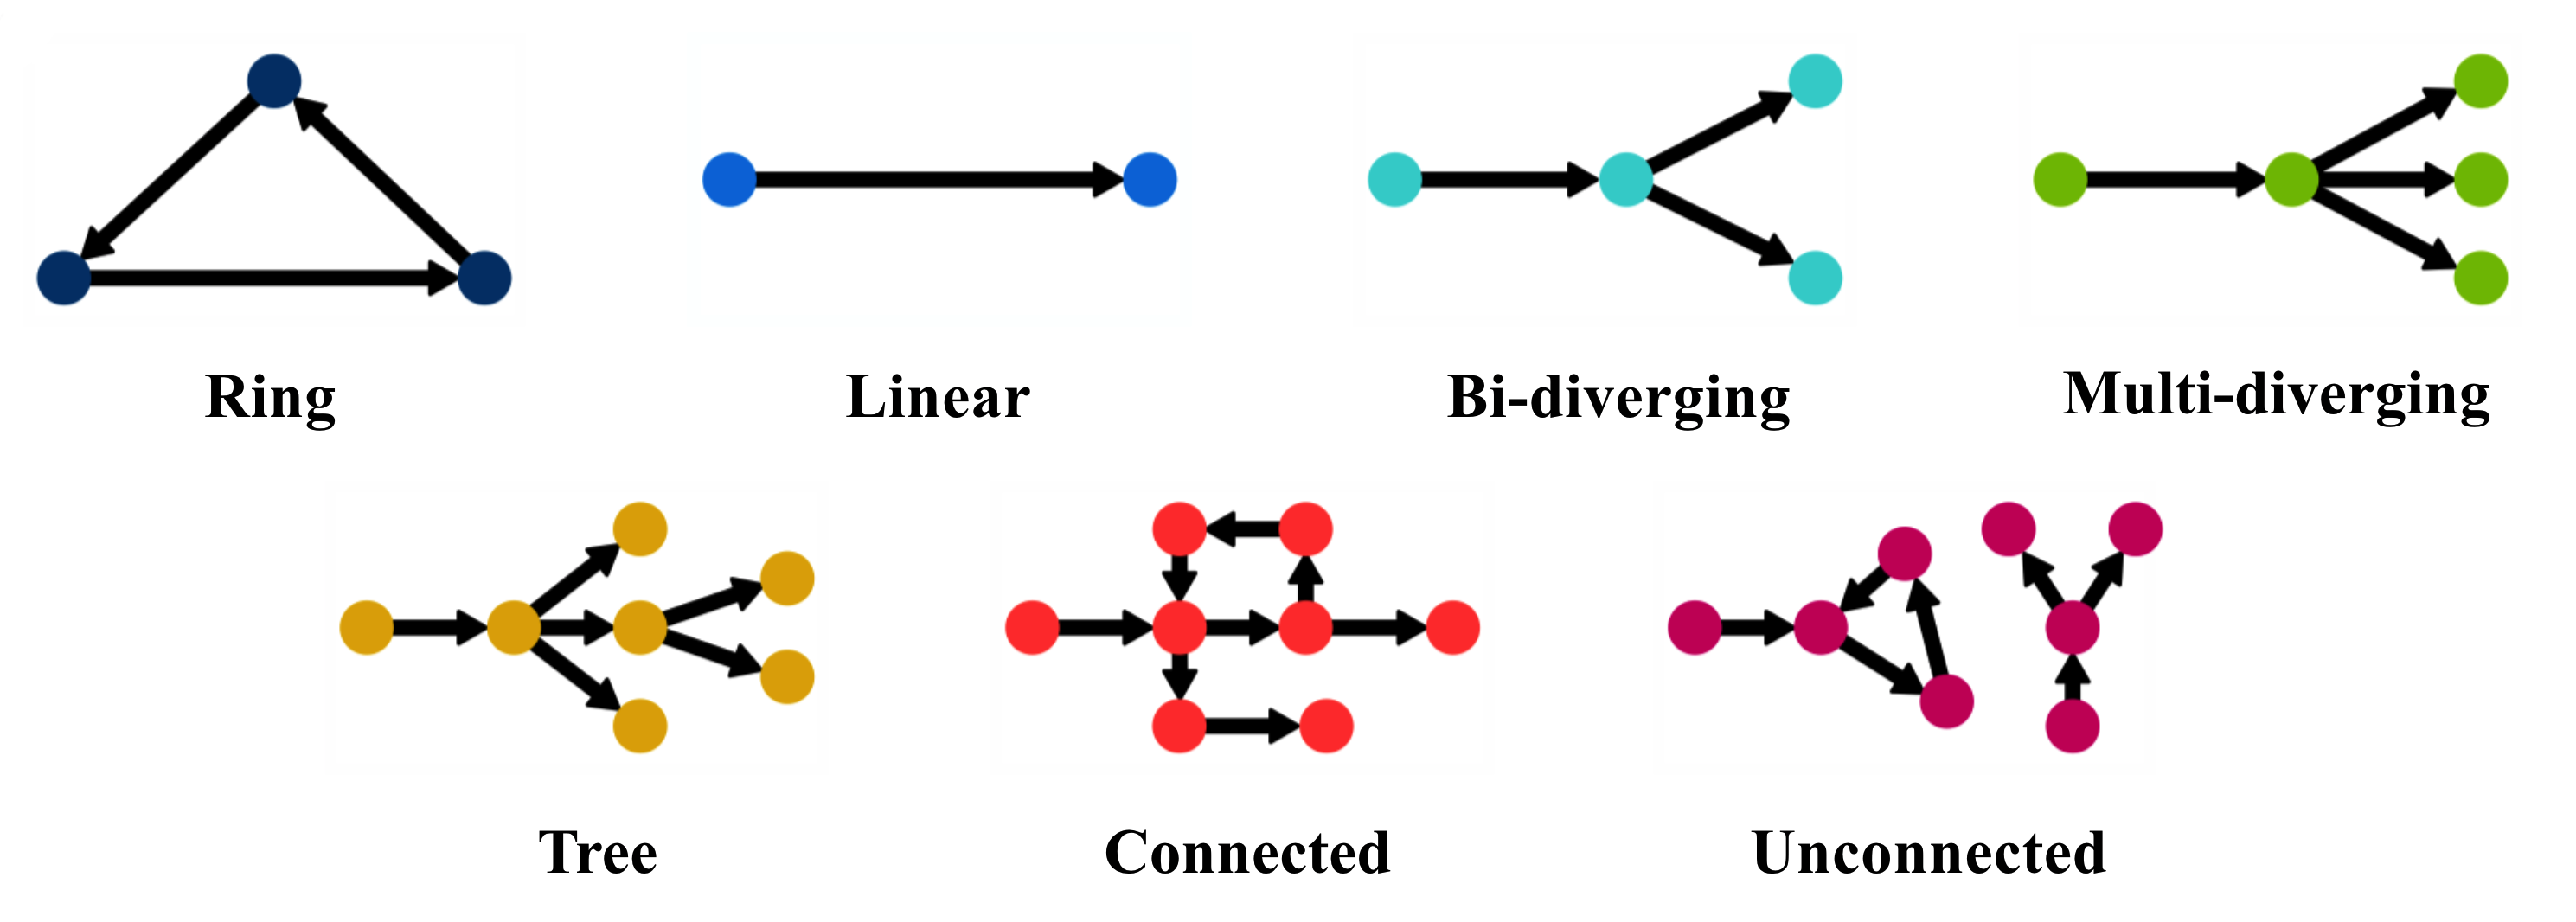
\includegraphics[width=1\linewidth]{Figures/types.png}
\caption{Seven basic trajectory structure types}
\label{fig:Trajectory}
\end{figure}


\subsection{Inferable Trajectory Structures of scTI Methods}
\newcommand{\Able}{\blacksquare}
\newcommand{\Unab}{\square}
\begin{spacing}{1.16}
\begin{table}[H]
\caption{Inferable Trajectory Structures of scTI Methods}
\label{tab:Inferable Trajectory}
\centering
\begin{tabular}{p{4cm} *{7}{p{1cm}<{\centering}}}
% \times \checkmark
\toprule
\tabhead{Method} & \tabhead{R} & \tabhead{L} & \tabhead{B} & \tabhead{M} 
                 & \tabhead{T} & \tabhead{C} & \tabhead{U} \\
\midrule
\multicolumn{2}{l}{\keyword{Tree}} \\
Monocle\_1   &$\Unab$&$\Able$&$\Able$&$\Able$&$\Able$&$\Unab$&$\Unab$ \\
Monocle\_2   &$\Unab$&$\Able$&$\Able$&$\Able$&$\Able$&$\Unab$&$\Unab$ \\
Slingshot    &$\Unab$&$\Able$&$\Able$&$\Able$&$\Able$&$\Unab$&$\Unab$ \\
MST          &$\Unab$&$\Able$&$\Able$&$\Able$&$\Able$&$\Unab$&$\Unab$ \\
SCUBA        &$\Unab$&$\Able$&$\Able$&$\Able$&$\Able$&$\Unab$&$\Unab$ \\
pCreode      &$\Unab$&$\Able$&$\Able$&$\Able$&$\Able$&$\Unab$&$\Unab$ \\
\midrule
\multicolumn{2}{l}{\keyword{Linear}} \\
Embeddr      &$\Unab$&$\Able$&$\Unab$&$\Unab$&$\Unab$&$\Unab$&$\Unab$ \\
TSCAN        &$\Unab$&$\Able$&$\Unab$&$\Unab$&$\Unab$&$\Unab$&$\Unab$ \\
SCORPIU      &$\Unab$&$\Able$&$\Unab$&$\Unab$&$\Unab$&$\Unab$&$\Unab$ \\
Component\_1 &$\Unab$&$\Able$&$\Unab$&$\Unab$&$\Unab$&$\Unab$&$\Unab$ \\
MATCHER      &$\Unab$&$\Able$&$\Unab$&$\Unab$&$\Unab$&$\Unab$&$\Unab$ \\
\midrule
\multicolumn{2}{l}{\keyword{Multi-diverging}} \\
STEMNET      &$\Unab$&$\Unab$&$\Able$&$\Able$&$\Unab$&$\Unab$&$\Unab$ \\
MFA          &$\Unab$&$\Able$&$\Able$&$\Able$&$\Unab$&$\Unab$&$\Unab$ \\
FateID       &$\Unab$&$\Unab$&$\Able$&$\Able$&$\Unab$&$\Unab$&$\Unab$ \\
\midrule
\multicolumn{2}{l}{\keyword{Bi-diverging}} \\
DPT          &$\Unab$&$\Unab$&$\Able$&$\Unab$&$\Unab$&$\Unab$&$\Unab$ \\
Wishbone     &$\Unab$&$\Able$&$\Able$&$\Unab$&$\Unab$&$\Unab$&$\Unab$ \\
\midrule
\multicolumn{2}{l}{\keyword{Graph}} \\
RaceID       &$\Able$&$\Able$&$\Able$&$\Able$&$\Able$&$\Able$&$\Able$ \\
PAGA         &$\Able$&$\Able$&$\Able$&$\Able$&$\Able$&$\Able$&$\Able$ \\
\midrule
\multicolumn{2}{l}{\keyword{Cyclic}} \\
EIPiGraph    &$\Able$&$\Unab$&$\Unab$&$\Unab$&$\Unab$&$\Unab$&$\Unab$ \\
Angle        &$\Able$&$\Unab$&$\Unab$&$\Unab$&$\Unab$&$\Unab$&$\Unab$ \\
% ${\rm R^{2}_{i}}$ 改成正常体
\bottomrule
\end{tabular}
\end{table}
\keyword{R} : Ring structure,     \keyword{L} : Linear structure, \\
\keyword{B} : Bi-diverging structure,      \keyword{M} : Multi-diverging structure, \\
\keyword{T} : Tree structure,     \keyword{C} : Connected structure, 
\keyword{U} : Unconnected structure \\
$\Able$ : This method is able to infer this kind of trajectory structure. \\
$\Unab$ : This method is not able to infer this kind of trajectory structure.
\end{spacing}






%----------------------------------------------------------------------------------------



%----------------------------------------------------------------------------------------




%The \code{biblatex} package is used to format the bibliography and inserts references such as this one \parencite{Reference1}. The options used in the \file{main.tex} file mean that the in-text citations of references are formatted with the author(s) listed with the date of the publication. Multiple references are separated by semicolons (e.g. \parencite{Reference2, Reference1}) and references with more than three authors only show the first author with \emph{et al.} indicating there are more authors (e.g. \parencite{Reference3}). This is done automatically for you. To see how you use references, have a look at the \file{Chapter1.tex} source file. Many reference managers allow you to simply drag the reference into the document as you type.

